\documentclass{beamer}
\usepackage{listings}
\lstset{
%language=C,
frame=single, 
breaklines=true,
columns=fullflexible
}
\usepackage{subcaption}
\usepackage{url}

\usepackage{tikz}
\usepackage{pgfplots}
\pgfplotsset{compat=1.17}
\usepackage{tkz-fct}
\usepackage{mathrsfs}
\usepackage{txfonts}
\usepackage{tkz-euclide} 
\usetikzlibrary{calc,math}
\usepackage{float}
\newcommand\norm[1]{\left\lVert#1\right\rVert}
\renewcommand{\vec}[1]{\mathbf{#1}}
\providecommand{\pr}[1]{\ensuremath{\Pr\left(#1\right)}}
\usepackage[export]{adjustbox}
\usepackage[utf8]{inputenc}
\usepackage{amsmath}
\usetheme{Boadilla}
\title{Research Paper Presentation}
\author{Aman Panwar - CS20BTECH11004}

\providecommand{\erfc}[1]{\ensuremath{\text{erfc}\left(#1\right)}}


\newcommand{\Integral}[2]{\ensuremath{\int\limits_{#1}^{#2}}}
\providecommand{\mbf}{\mathbf}
\providecommand{\pr}[1]{\ensuremath{\Pr\left(#1\right)}}
\providecommand{\qfunc}[1]{\ensuremath{Q\left(#1\right)}}
\providecommand{\sbrak}[1]{\ensuremath{{}\left[#1\right]}}
\providecommand{\lsbrak}[1]{\ensuremath{{}\left[#1\right.}}
\providecommand{\rsbrak}[1]{\ensuremath{{}\left.#1\right]}}
\providecommand{\brak}[1]{\ensuremath{\left(#1\right)}}
\providecommand{\lbrak}[1]{\ensuremath{\left(#1\right.}}
\providecommand{\rbrak}[1]{\ensuremath{\left.#1\right)}}
\providecommand{\cbrak}[1]{\ensuremath{\left\{#1\right\}}}
\providecommand{\lcbrak}[1]{\ensuremath{\left\{#1\right.}}
\providecommand{\rcbrak}[1]{\ensuremath{\left.#1\right\}}}
\theoremstyle{remark}
\newtheorem{rem}{Remark}
\newcommand{\sgn}{\mathop{\mathrm{sgn}}}
\providecommand{\abs}[1]{\vert#1\vert}
\providecommand{\res}[1]{\Res\displaylimits_{#1}} 
\providecommand{\norm}[1]{\lVert#1\rVert}
%\providecommand{\norm}[1]{\lVert#1\rVert}
\providecommand{\mtx}[1]{\mathbf{#1}}
\providecommand{\mean}[1]{E[ #1 ]}
\providecommand{\fourier}{\overset{\mathcal{F}}{ \rightleftharpoons}}
%\providecommand{\hilbert}{\overset{\mathcal{H}}{ \rightleftharpoons}}
\providecommand{\system}{\overset{\mathcal{H}}{ \longleftrightarrow}}
	%\newcommand{\solution}[2]{\textbf{Solution:}{#1}}
\providecommand{\dec}[2]{\ensuremath{\overset{#1}{\underset{#2}{\gtrless}}}}
\newcommand{\myvec}[1]{\ensuremath{\begin{pmatrix}#1\end{pmatrix}}}
\newcommand{\mydet}[1]{\ensuremath{\begin{vmatrix}#1\end{vmatrix}}}
\numberwithin{equation}{subsection}
\makeatletter
\@addtoreset{figure}{problem}
\makeatother
\let\StandardTheFigure\thefigure
\let\vec\mathbf
\renewcommand{\thefigure}{\theproblem}
\def\putbox#1#2#3{\makebox[0in][l]{\makebox[#1][l]{}\raisebox{\baselineskip}[0in][0in]{\raisebox{#2}[0in][0in]{#3}}}}
     \def\rightbox#1{\makebox[0in][r]{#1}}
     \def\centbox#1{\makebox[0in]{#1}}
     \def\topbox#1{\raisebox{-\baselineskip}[0in][0in]{#1}}
     \def\midbox#1{\raisebox{-0.5\baselineskip}[0in][0in]{#1}}
\vspace{3cm}
\newcommand\tab[1][1cm]{\hspace*{#1}}
\begin{document}
\begin{frame}
\titlepage
\end{frame}


\section{Introduction}

\begin{frame}
\frametitle{BER Analysis of a NOMA Enhanced Backscatter Communication System}
\begin{block}{Abstract}
    \begin{enumerate}
        \item Analyses the BER performance of a NOMA enhanced BackCom system with imperfect SIC. One reader and two BNs are considered.
        \item Compares the effective non-errornous transmitted bits over a large period in NOMA vs OMA
        \item Derives equation for optimal reflection coefficients for the two BNs
    \end{enumerate}
\end{block}
\end{frame}

\begin{frame}
\frametitle{Introduction}
\begin{block}{Keywords}
    \begin{enumerate}
        \item \textbf{BackCom: } Backscatter Communication
        \item \textbf{BN: } Backscatter Node
        \item \textbf{BER: } Bit Error Rate
        \item \textbf{NOMA: } Non-Orthogonal Multiple Access
        \item \textbf{BSPK: } Binary Phase Shift Keying
        \item \textbf{AWGN: } Additive White Gaussian Noise
        \item \textbf{SIC: } Successive Interference Cancellation
    \end{enumerate}
\end{block}
\end{frame}


\section{System Model}

\begin{frame}
\frametitle{System Model}
\begin{block}{Figure}
    \begin{figure}
    \centering
    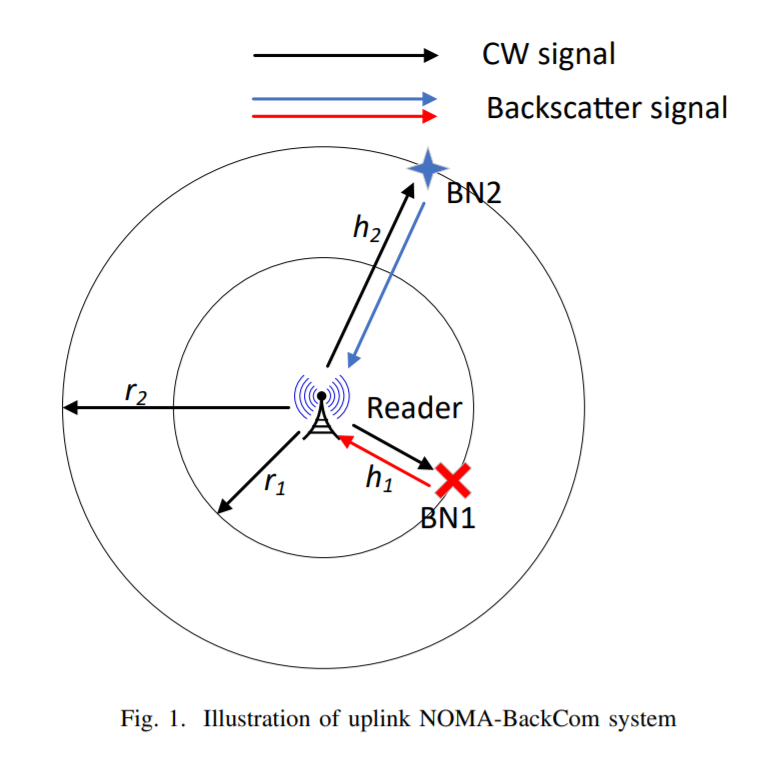
\includegraphics[scale=0.35]{fig.png}
    \label{fig:my_label}
\end{figure}
\end{block}
\end{frame}

\begin{frame}
\frametitle{System Model}
\begin{block}{Important Formulae}
    The signal received by the reader is
    \begin{align}
        y&=\sqrt{P_r \xi_1}h_1 x_1 + \sqrt{P_r \xi_2}h_2 x_2 + w\nonumber
    \end{align}
    Here,\\
    \tab $P_r$ is reader transmitted power\\
    \tab $\xi_i$ are the power reflection coefficient\\
    \tab $h_i$ are channel coefficients b/w BNs and reader\\
    \tab $x_i$ is the BPSK modulated information signal of BNi\\
    \tab $w$ is the AWGN with 0 mean and $N_0$ varinace
    
    
    (A strong line-of-sight is assumed in this model. Also, the BNs are numbered such that $\xi_1 > \xi_2$)
\end{block}
\end{frame}

\begin{frame}
\frametitle{System Model}
\begin{block}{BER for User 1}
    Probability that the bit read from the first BN has error
    \begin{align}
        P_1(e) = \frac{1}{4}\brak{\erfc{ \frac{\srqt{\epsilon_b \xi_1}+\sqrt{\brak{\epsilon_b \xi_1}/R } }{N_0} } + \erfc{ \frac{\srqt{\epsilon_b \xi_1}-\sqrt{\brak{\epsilon_b \xi_1}/R } }{N_0} }}\nonumber
    \end{align}
    where $\erfc{}$ is the complementary error function
    \begin{align}
        \erfc{z}&=\frac{2}{\sqrt{\pi}}\Integral{z}{\infty}e^{-t^{2}} d t\nonumber
    \end{align}
\end{block}
\end{frame}

\begin{frame}
\frametitle{System Model}
\begin{block}{BER for User 2}
    NOMA uses SIC i.e. to recognise the second signal, the first signal is subtracted from the received signal. Thus, probability of error in second signal depend on $P_1$
    
    When first signal is correctly decoded,
    \begin{align}
        P_{2(I)}&=\frac{1}{4}\brak{ 2\erfc{ \sqrt{ \frac{\brak{\epsilon_b \xi_1}/R}{N_0} } } - \erfc{ \frac{\sqrt{\epsilon_b \xi_1}+\sqrt{\brak{\epsilon_b \xi_1}/R}}{\sqrt{N_0}} } }\nonumber
    \end{align}
    When first signal is incorrectly decoded,
    \begin{align}
        P_{2(II)}&=\frac{1}{4}\brak{ 
        \erfc{ \frac{2\sqrt{\epsilon_b \xi_1}+\sqrt{\brak{\epsilon_b \xi_1}/R}}{\sqrt{N_0}} } 
        +\erfc{ \frac{\sqrt{\epsilon_b \xi_1}-\sqrt{\brak{\epsilon_b \xi_1}/R}}{\sqrt{N_0}} }\nonumber\\
        &-\erfc{ \frac{2\sqrt{\epsilon_b \xi_1}-\sqrt{\brak{\epsilon_b \xi_1}/R}}{\sqrt{N_0}} }}\nonumber
    \end{align}
\end{block}
\end{frame}


\begin{frame}
\frametitle{System Model}
\begin{block}{BER for User 2}
    The final probability of error in bit read from the second user
    \begin{align}
        P_2 &= \frac{1}{4}\brak{ 2\erfc{ \sqrt{ \frac{\brak{\epsilon_b \xi_1}/R}{N_0} } } - \erfc{ \frac{\sqrt{\epsilon_b \xi_1}+\sqrt{\brak{\epsilon_b \xi_1}/R}}{\sqrt{N_0}} }\nonumber\\
        &+\erfc{ \frac{2\sqrt{\epsilon_b \xi_1}+\sqrt{\brak{\epsilon_b \xi_1}/R}}{\sqrt{N_0}} } 
        +\erfc{ \frac{\sqrt{\epsilon_b \xi_1}-\sqrt{\brak{\epsilon_b \xi_1}/R}}{\sqrt{N_0}} }\nonumber\\
        &-\erfc{ \frac{2\sqrt{\epsilon_b \xi_1}-\sqrt{\brak{\epsilon_b \xi_1}/R}}{\sqrt{N_0}} }}\nonumber
    \end{align}
\end{block}
\end{frame}

\section{Simulations}
\begin{frame}
\frametitle{Simulation Result}
\begin{block}{Simulation 1: BER vs SNR}
\begin{figure}
    \centering
    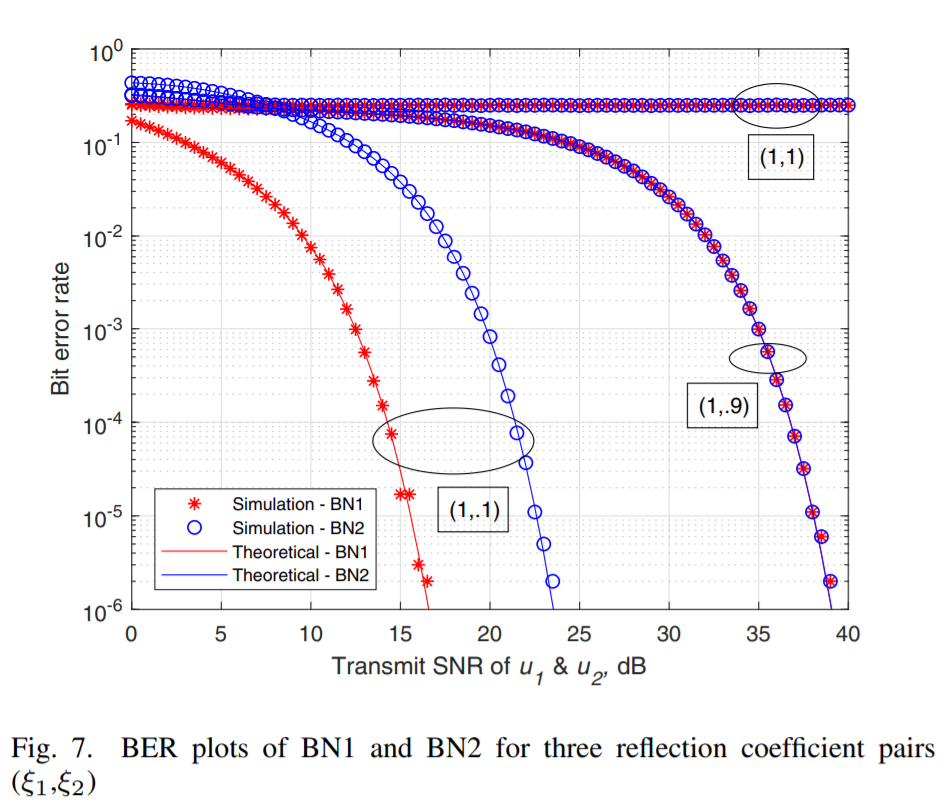
\includegraphics[scale=0.27]{sim1.png}
    \label{fig:my_label}
\end{figure}
Greater separation in reflection coefficients($\xi_1$ and $\xi_2$) leads to smaller BER. This is due to decreased inter-user interface(IUI).
\end{block}
\end{frame}

\begin{frame}
\frametitle{Simulation Result}
\begin{block}{Simulation 2: Effective bits transfered vs SNR for NOMA and OMA}
\begin{figure}
    \centering
    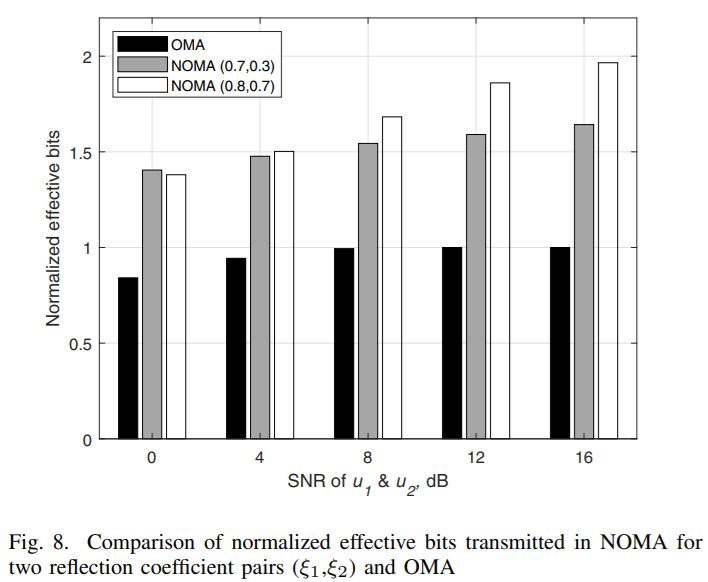
\includegraphics[scale=0.27]{sim2.png}
    \label{fig:my_label}
\end{figure}
\begin{enumerate}
    \item This simulation shows that NOMA does outperform OMA-TDMA (Orthogonal Multiple Access - Time Division Multiple Access)
    \item The separation in reflection coefficients greatly effect the no. of correctly transmission of bits.
\end{enumerate}

\end{block}
\end{frame}


\begin{frame}
\frametitle{Simulation Result}
\begin{block}{Simulation 3: $\xi_1$ vs $\xi_2$ for specific BER}
\begin{figure}
    \centering
    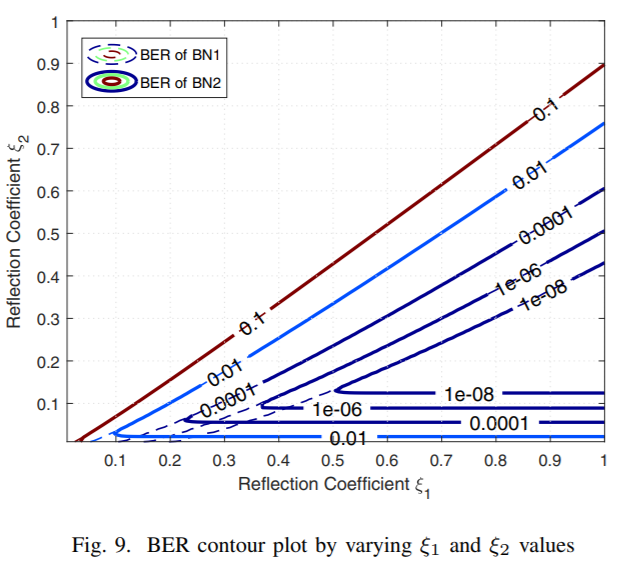
\includegraphics[scale=0.27]{sim3.png}
    \label{fig:my_label}
\end{figure}
\begin{enumerate}
    \item Only a small range of $\xi_2$ achieves acceptable performance.
    \item BER performance of BN1 is independent of $\xi_2$
\end{enumerate}
\end{block}
\end{frame}

\begin{frame}
\frametitle{Simulation Result}
\begin{block}{Simulation 3: $\xi_1$ vs $\xi_2$ for specific BER}

\begin{table}[]
    \centering
    \renewcommand{\arraystretch}{1.3}
    \begin{tabular}{|c|p{0.2\columnwidth}|}
    \hline
    Parameter & Value\\ \hline
        P_r&20dBm\\ \hline
        N_0&-90dBm\\ \hline
        Path loss exponent&2\\ \hline
        r_1& 25m\\ \hline
        r_2& 25m \\ \hline
        Effective SNR & 24.08 dB \\ \hline
    \end{tabular}
    \caption{Simulation Parameters}
    \label{tab:my_label_2}
\end{table}

\end{block}
\end{frame}




\begin{frame}
\frametitle{Simulation Result}
\begin{block}{Simulation 4: Effective bits transfered vs SNR for NOMA and OMA}
\begin{figure}
    \centering
    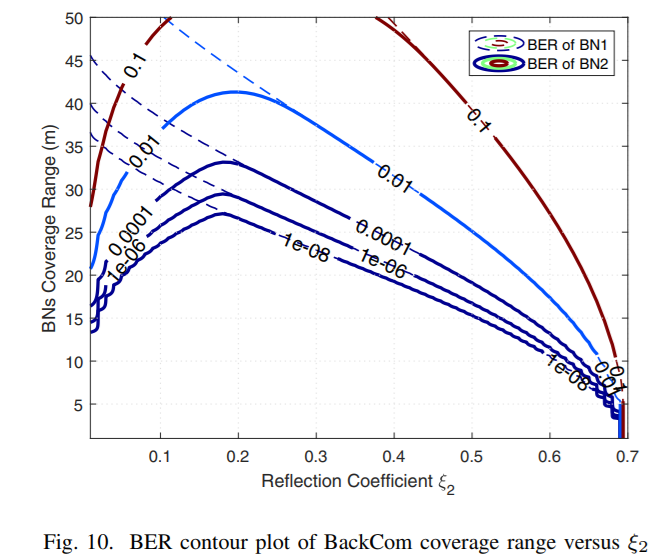
\includegraphics[scale=0.27]{sim4.png}
    \label{fig:my_label}
\end{figure}
\begin{enumerate}
    \item In this given case, the optimal $\xi_2$ is about one-fourth of $\xi_1$.
    \item If $\xi_1=0.7$, QoS requirement of BER is $10^{-3}$ and coverage range is 33m then optimal $\xi_2 = 0.19$ 
\end{enumerate}

\end{block}
\end{frame}
\begin{frame}
\frametitle{Simulation Result}
\begin{block}{Simulation 4: Effective bits transfered vs SNR for NOMA and OMA}

\begin{table}[]
    \centering
    \renewcommand{\arraystretch}{1.3}
    \begin{tabular}{|c|p{0.2\columnwidth}|}
    \hline
    Parameter & Value\\ \hline
        P_r&20dBm\\ \hline
        N_0&-90dBm\\ \hline
        Path loss exponent&2\\ \hline
        r_1& 25m\\ \hline
        r_2& 25m \\ \hline
        Effective SNR & 24.08 dB \\ \hline
        \xi_1 & 0.7 \\ \hline
    \end{tabular}
    \caption{Simulation Parameters}
    \label{tab:my_label_2}
\end{table}
\end{block}
\end{frame}


\begin{frame}
\frametitle{Conclusion}
\begin{block}{Conclusion}
\begin{enumerate}
    \item  The numerical results are found to match perfectly
with Monte Carlo simulations
    \item Moreover, derived BER expressions have been evaluated for different reflection coefficients and ranges to find optimum values for each scenario
    \item NOMA has a upper hand over OMA when it comes to BackCom
\end{enumerate}
\end{block}
\end{frame}


\end{document}
